\begin{frame}{Les termes}
  \begin{columns}
    \begin{column}{0.65\textwidth}
      \begin{block}{}
        \begin{itemize}[<+->]
        \item Des symboles d'arité fixe : $f^{\backslash 2}$
        \item Un alphabet : $\{ a^{\backslash 0}, b^{\backslash 0}, s^{\backslash 1}, h^{\backslash 1}, f^{\backslash 2}\}$
        \item Un terme : $f(f(s(a), a),s(f(b,b)))$
        \end{itemize}
      \end{block}
    \end{column}
    \begin{column}{0.35\textwidth}
      \onslide<4>
      \begin{center}
        \begin{tikz}
          \node {$f$}
          child { node {$f$}
            child { node {$s$}
              child { node {$a$} } }
            child { node {$a$} } }
          child { node {$s$}
            child {node {$f$}
              child { node {$b$} }
              child { node {$b$} } } };
        \end{tikz}
      \end{center}
    \end{column}
  \end{columns}
\end{frame}

\begin{frame}{Langages formels}
  Un ensemble de termes
  \begin{block}{}
    \begin{itemize}[<+->]
    \item Langages réguliers : $\{f(s^*(a),s^*(a))\}$
    \item Langages synchronisés : $\{f(s^n(a),s^n(a)) \mid n \geq 0\}$
    \item Langages algébriques : $\{s^n(h^n(a)) \mid n \geq 0\}$
    \item Langages synchronisés algébriques : $\{f(s^n(h^n(a)),s^n(h^n(b))) \mid n \geq 0\}$
    \end{itemize}
  \end{block}
  \vspace{\baselineskip}
  \begin{overprint}
    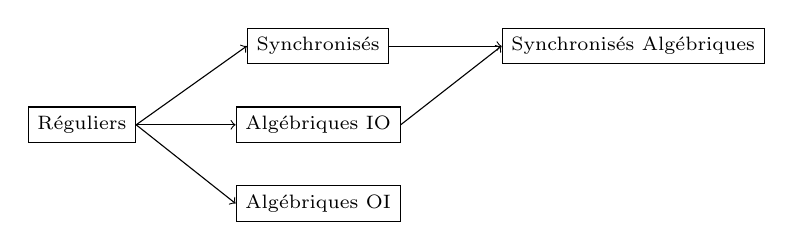
\begin{tikzpicture}

      \tikzstyle{language} = [shape=rectangle, draw];
      
      \onslide<1->{
        \node[language] (reg) at (0,0) {\scriptsize{Réguliers}};
      }

      \onslide<2->{
        \node[language] (synch) at (3,1) {\scriptsize{Synchronisés}};
        \draw[->] (reg.east) -- (synch.west);
      }

      \onslide<3->{
        \node[language] (algeio) at (3,0) {\scriptsize{Algébriques IO}};
        \node[language] (algeoi) at (3,-1) {\scriptsize{Algébriques OI}};
        \draw[->] (reg.east) -- (algeio.west);
        \draw[->] (reg.east) -- (algeoi.west);
      }

      \onslide<4->{
        \node[language] (synchalge) at (7,1) {\scriptsize{Synchronisés Algébriques}};
        \draw[->] (synch.east) -- (synchalge.west);
        \draw[->] (algeio.east) -- (synchalge.west);
      }
    \end{tikzpicture}
  \end{overprint}
\end{frame}

\begin{frame}{Variables}
  \begin{columns}
    \begin{column}{0.6\textwidth}
      \begin{itemize}
      \item<1-> Ensemble de variables : $\mathcal X = \{x, y\}$
      \item<2-> La substitution : $\sigma = (x / s(b))$
      \item<4-> Le filtrage : $\sigma(t) = t'$
      \item<6-> L'unification : $\alpha(t) = \alpha(t')$
      \end{itemize}
    \end{column}
    \begin{column}{0.4\textwidth}
      \begin{overprint}
        \onslide<2-3>
        \begin{center}
          $t = f(x,s(a))$\\
          \begin{tikzpicture}[level distance = 1cm]
            \node {$f$}
            child { node {$x$}}
            child { node {$s$}
              child {node {$a$}}};
          \end{tikzpicture}
        \end{center}
        \onslide<4-5>
        \begin{center}
          $t = f(x,s(a))$\\
          \begin{tikzpicture}[level distance = 1cm]
            \node {$f$}
            child { node {$x$}}
            child { node {$s$}
              child {node {$a$}}};
          \end{tikzpicture}
        \end{center}
        \onslide<6->
        \begin{center}
          \begin{columns}
            \begin{column}{0.5\textwidth}
              $t = f(x,s(a))$\\
              \begin{tikzpicture}[level distance = 1cm]
                \node {$f$}
                child { node {$x$}}
                child { node {$s$}
                  child {node {$a$}}};
              \end{tikzpicture}
            \end{column}
            \begin{column}{0.5\textwidth}
              $t' = f(s(b),y)$\\
              \begin{tikzpicture}[level distance = 1cm]
                \node {$f$}
                child { node {$s$}
                  child {node {$b$}}}
                child { node {$y$}};
              \end{tikzpicture}
            \end{column}
          \end{columns}
        \end{center}
      \end{overprint}
      
      \begin{overprint}
        \onslide<3>
        \begin{center}
          $\sigma(t) = f(s(b),s(a))$\\
          \begin{tikzpicture}[level distance = 1cm]
            \node {$f$}
            child { node {$s$}
              child {node {$b$}}}
            child { node {$s$}
              child {node {$a$}}};
          \end{tikzpicture}
        \end{center}
        \onslide<5>
        \begin{center}
          $t' = f(s(b),s(a))$\\
          \begin{tikzpicture}[level distance = 1cm]
            \node {$f$}
            child { node {$s$}
              child {node {$b$}}}
            child { node {$s$}
              child {node {$a$}}};
          \end{tikzpicture}
        \end{center}
        \onslide<7>
        \begin{center}
          $\alpha(t) = \alpha(t') = f(s(b),s(a))$\\
          $\alpha = (x/s(b), y/s(a))$\\
          \begin{tikzpicture}[level distance = 1cm]
            \node {$f$}
            child { node {$s$}
              child {node {$b$}}}
            child { node {$s$}
              child {node {$a$}}};
          \end{tikzpicture}
        \end{center}
      \end{overprint}
    \end{column}
  \end{columns}
\end{frame}

\begin{frame}{Systèmes de réécriture}
  \begin{itemize}
  \item $r$ et $l$ des termes
  \item $Var(r) \subseteq Var(l)$
  \item $l \rightarrow r$ est une règle de réécriture
  \end{itemize}
  \begin{center}
    $s(x) \rightarrow s(s(x))$\\
    $t = f(b,s(a))$\\
    \onslide<2->
    $\sigma(s(x)) = s(a)$ avec $\sigma = (x / a)$\\
    \onslide<3->
    $t \rightarrow t'$ \\
    \onslide<5>
    $t' = f(b,s(s(a)))$ \\
    \onslide<1->
    \begin{overprint}
      \onslide<1-3>
      \begin{center}
        \begin{tikzpicture}[level distance = 1cm]
          \node {$f$}
          child { node {$b$}}
          child { node {$s$}
            child {node {$a$}}};
        \end{tikzpicture}
      \end{center}
      \onslide<4>
      \begin{center}
        \begin{tikzpicture}[level distance = 1cm]
          \node {$f$}
          child { node {$b$}}
          child { node {$s$}
            child { node {$s$}
              child {node {$x$}}}};
        \end{tikzpicture}
      \end{center}
      \onslide<5>
      \begin{center}
        \begin{tikzpicture}[level distance = 1cm]
          \node {$f$}
          child { node {$b$}}
          child { node {$s$}
            child { node {$s$}
              child {node {$a$}}}};
        \end{tikzpicture}
      \end{center}
    \end{overprint}
  \end{center}
\end{frame}
